\chapter{THERMAL EQUILIBRIUM}
% !TEX root = hazy3.tex

\section{Overview}

This section describes the system of equations setting the local thermal
balance of a cloud.  The electron temperature is the only thermodynamic
quantity used to characterize a photoionized cloud.  The electron velocity
distribution is predominantly Maxwellian \citep{Bohm1947} although
a trace constituent of non-thermal electrons may contribute when high-energy
photons are present (\citealp{Spitzer1968}).  A kinetic temperature can
then characterize most of the electron velocity distribution.  This in turn
is defined by the balance between processes that add energy (heat) and remove
energy (cool) the electrons.

Heating or cooling can be defined relative to either the ground state
or continuum, and this difference has caused some confusion in the
literature.  \Cloudy\ defines heating and cooling relative to the continuum AGN3).
Note that, in this scheme of bookkeeping,
photoionization contributes an amount of heat given by $h(\nu-\nu_o$),
where $h\nu_o$
is the ionization potential of the atom or ion and $\nu$ is the photon energy.
Emission of a recombination line \emph{does not} constitute a cooling process.
Heating and cooling rates are computed in cgs units (ergs, not Rydbergs)
throughout \Cloudy.

\section{Thermal stability}

The criterion for thermal stability used by \Cloudy\ is that the net cooling
(i.e., cooling minus heating) has a positive temperature derivative (\citealp{Field1965}).  This can be expressed as
\begin{equation}
\label{eqn:ThermalStability}
\frac{{d\left( {\Lambda  - G} \right)}}{{dT}} > 0.% (1)
\end{equation}

The code will print a ``u'' next to the temperature in the zone results,
and make a comment at the end of the calculation, if possibly thermally
unstable solutions were found. The criterion used by the code is that the
derivative \emph{at constant density} (isochoric) be positive.  The more traditional
criterion is that the derivative \emph{at constant pressure} (isobaric) be positive
(\citealp{Field1965}).

The fact that the code identifies a region as possibly thermally unstable
does not necessarily show that it is.  The derivatives used in equation
\ref{eqn:ThermalStability} are those found during the search for the thermal solution.  As such they
are evaluated out of equilibrium as part of the temperature solver.
Their
primary purpose was not to perform this thermal stability analysis.  A
section of Part III of this document goes into more detail about the
stability check performed by the code, and how to do a better one.

\section{Compton energy exchange}

There are two parts to the Compton energy exchange problem.  First,
photons scatter off an electron at an angle $\theta$, causing a change of photon
energy due to Compton recoil given by
\begin{equation}
\label{eqn:ComptonEnergyShift}
\frac{{\Delta {\varepsilon _ - }}}{{{\varepsilon _o}}} = \left[ {1 -
\frac{1}{{1 + \left( {{\varepsilon _o}/{m_e}{c^2}} \right)\left( {1 - \cos
\theta } \right)}}} \right].
\end{equation}
For isotropic scattering the median scattering angle corresponds to
$cos \theta = 0.5$.  Scattering by thermal electrons crates a shift with a distribution
centered at
\begin{equation}
\frac{{\Delta {\varepsilon _ - }}}{{{\varepsilon _o}}} =
\frac{{4kT}}{{{m_e}{c^2}}}
\end{equation}
and a standard deviation given by
\begin{equation}
\frac{\sigma }{{{\varepsilon _o}}} = \sqrt {\frac{{2kT}}{{{m_e}{c^2}}}}
\end{equation}
(see, e.g., \citealp{Zycki1994}).

The net volume-heating rate due to Compton energy exchange is given by
\begin{equation}
\label{eqn:ComptonEnergyExchange}
{G_{Comp}} - {\Lambda _{Comp}} = \frac{{4\pi \,{n_e}}}{{{m_e}{c^2}}}\left\{
{\int {{\sigma _h}{J_\nu }h\nu \left[ {1 + {\eta _\nu }} \right]} \;d\nu
- 4kT\int {{\sigma _c}{J_\nu }\;d\nu } } \right\}\quad [\mathrm{erg~s}^{-1}
\mathrm{cm}^{-3}]
\end{equation}
See, for instance, \citep{Levich1970} and \citep{Krolik1981}.  The two terms in braces are the heating and cooling terms
respectively, while the factor in brackets in the first term accounts for
heating due to both spontaneous and stimulated Compton scattering.  Induced
Compton heating is important when $\eta_\nu$ is large at frequencies where
$h\nu\ge kT$.
In fact it is, at most, a few percent effect in most circumstances.

The terms $\sigma_h$ and $\sigma_c$ appearing in equation \ref{eqn:ComptonEnergyExchange} are the effective energy
exchange (scattering) cross section for energy exchange, and differ from
the Thomson cross section for energies $h\nu\sim m_e c^2$, where the Klein-Nishina
cross section must be used.
The numerical fits to the \citep{Winslow1975} results,
as used by \citep{Krolik1981} and kindly provided by Dr. C.B.
Tarter, are used.  Defining
\begin{equation}
\alpha  = {\left\{ {1 + {\nu _{Ryd}}\left( {1.1792 \times {{10}^{ - 4}}
+ 7.084 \times {{10}^{ - 10}}{\nu _{Ryd}}} \right)} \right\}^{ - 1}}
\end{equation}
and
\begin{equation}
\beta  = \left\{ {1 - \alpha {\nu _{Ryd}}\left( {1.1792 \times {{10}^{
- 4}} + 2 \times 7.084 \times {{10}^{ - 10}}{\nu _{Ryd}}} \right)/4}
\right\}\quad ,
\end{equation}
where $\nu_{Ryd}$ is the photon frequency in Rydbergs, the Compton energy-exchange
rate coefficients are then $\sigma_h = \sigma_T\alpha$  and $\sigma_c =
\sigma_T\alpha\beta$.
Tests show that these are
in excellent  (much better than 1\%) agreement with \citep{Guilbert1986}'s calculations for $h\nu < 10$~MeV,
the energies where Guilbert's calculations are valid.

The coefficients for the heating and cooling terms, i.e., $\alpha$ and the product
$\alpha\beta$, are calculated at the beginning of the calculation and stored in the
vectors \cdTerm{csigh}($\nu$) and \cdTerm{csigc}($\nu$).  The heating is determined by summing over
the continuum;
\begin{equation}
{G_{Comp}} = \frac{{{n_e}}}{{m{c^2}}}\;{\sigma _T}\;{\left( {h{\nu _{Ryd}}}
\right)^2}\;\sum {{\alpha _i}\;{\varphi _i}\;\nu _i^2\left( {1 + {\eta _i}}
\right)}
\end{equation}
where $\phi_i$ is the photon flux, $\eta_i$ is the photon occupation
number, $\sigma_T$ is the
Thomson cross section, and $\nu_i$ is the photon energy in Rydbergs .

Figure \ref{fig:ComptonEquilibriumError} shows results of a series of calculations in which Compton energy
exchange was the dominant physical process affecting the temperature.  These
are a series of models in which the gas was irradiated by black body continua
in strict thermodynamic equilibrium (i.e., $T_u = T_{color}$) and various hydrogen
densities.
Over the temperature range 3 K $\le T_{color}\le 10^{10}$~K the computed
equilibrium electron temperature equaled the color temperature within much
better than 1\% ($\left\langle {{T_e} - {T_{color}}} \right\rangle
/{T_{color}} =  - 0.00073 \pm 0.0019$).

\begin{figure}
\centering
\label{fig:ComptonEquilibriumError}
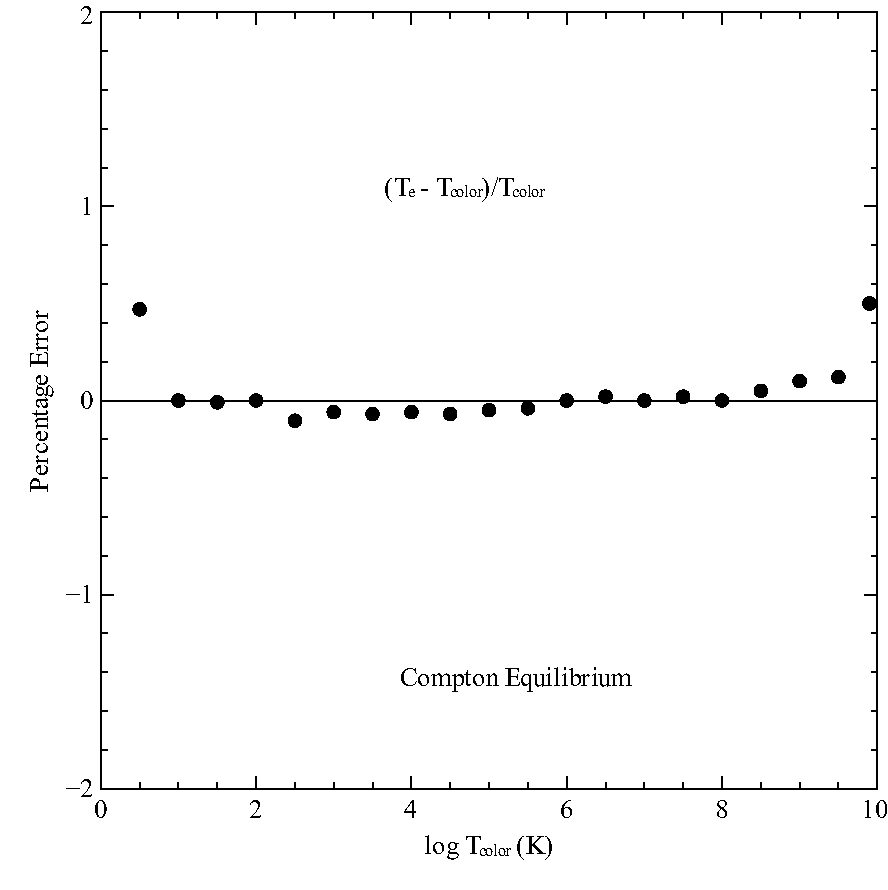
\includegraphics[scale=0.7]{ComptonEquilibriumError}
\caption[Compton Equilibrium Error]{Thermal equilibrium in the Compton Limit. Calculations are for
blackbody continua of various temperatures, given as $T_{color}$ along the x-axis.
The energy density temperature $T_u$ is set equal to $T_{color}$.  The density is
adjusted to maintain ionization parameters $U\sim  10^{10}$, so that the thermal
equilibrium equations are dominated by the Compton exchange problem.  The
deviation of the computed equilibrium temperature $T_e$ from the asymptotic
Compton temperature $T_{color}$ is shown.}
\end{figure}

The intended temperature range of validity for \Cloudy\ is \TEMPLIMITLOW $ -$\TEMPLIMITHIGH.  Over the more limited range $10 \K - 10^9 \K$ the computed Compton
 temperature, for conditions in which strict TE is expected, is generally
equal to the color temperature within three significant figures
(see Figure \ref{fig:ComptonEquilibriumError}).
At temperatures much greater than 10$^9$ K the electrons become
relativistic; \Cloudy\ is not intended for these conditions.  For temperatures
much less than 10 K the computed temperature fails high because the energy
bandwidth of the continuum array does not extend
below \emm .
As
a further test, the models presented by \citep{Krolik1981}
were recomputed with excellent agreement (typically within 3\%) with their
computed Compton temperatures.

For a blackbody radiation field with $T_u \ne T_{color}$ the Compton temperature
will not be equal to $_{Tcolor}$ because induced scattering will not contribute
the required amount of heating-cooling.  This case is shown in Figure
\ref{fig:ComptonSTE},
the results of a series of calculations in which the energy density
temperature was varied (this is shown as the x-axis), but the color
temperature held fixed at 10$^5$~K.

\begin{figure}
\centering
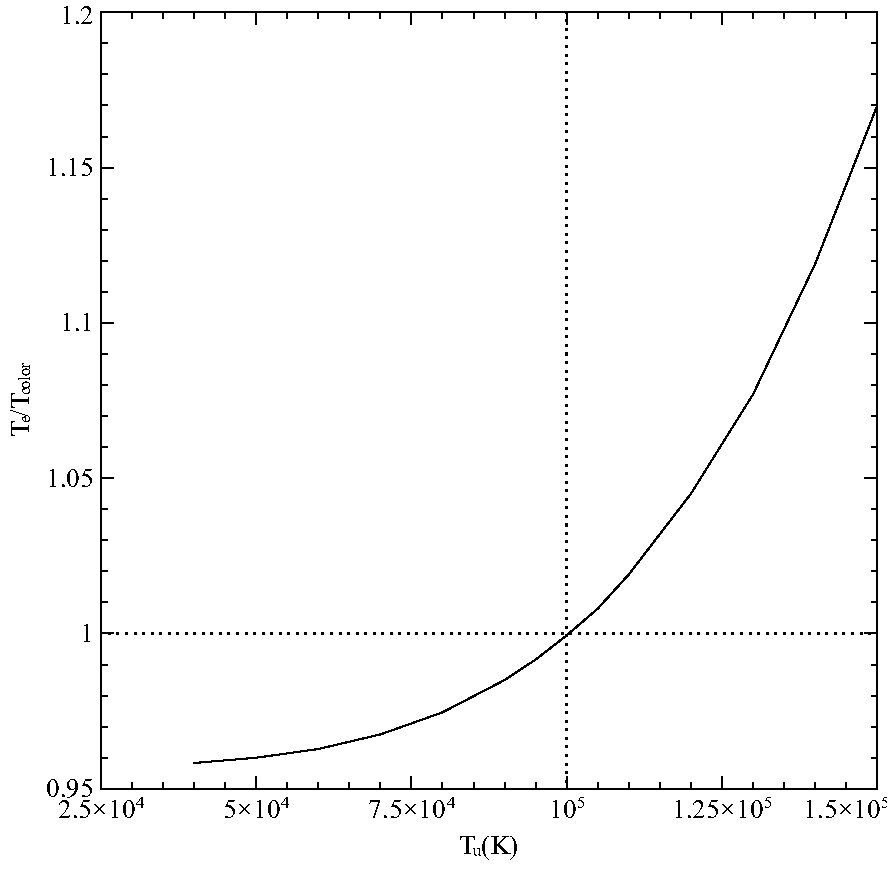
\includegraphics[scale=0.75]{ComptonSTE}
\label{fig:ComptonSTE}
\caption[Compton equilibrium in the STE limit]{Calculations are for 10$^5$ K blackbodies and various values of the
energy density temperature $T_u$, indicated along the x-axis. The ratio of
the computed equilibrium temperature $T_e$ to the color temperature
$T_{color}$
is shown.  The two are equal when the energy density and color temperatures
are equal. cmpnlte}
\end{figure}

Note also that when $T_u > T_{color}$ induced Compton heating
drives $T_e$ above $T_{color}$.
Only when the color and energy density temperatures are equal
do the equilibrium and color temperatures match.

\section{Bound Compton ionization, heating}

Compton scattering can ionize atoms for photons of sufficiently high
energy ($\approx 2.3$ keV for hydrogen).  The energy given to an electron
by a 90$^{\circ}$
scattering is found by rearranging equation \ref{eqn:ComptonEnergyShift}above
\begin{equation}
e = h\nu \left( {1 - \frac{1}{{1 + \frac{{h\nu }}{{m{c^2}}}}}} \right).
\end{equation}
Setting this equal to the ionization potential of the species, $h{\nu _o}$,
electrons will be removed by photons having an energy greater than
\begin{equation}
h\nu  = \sqrt {h{\nu _o}m{c^2}}.
\end{equation}

\section{Expansion cooling }

Adiabatic cooling (erg cm$^{-3}$ s$^{-1}$) due to the hydrodynamic expansion of
the gas is given by
\begin{equation}
{L_{\rm exp}} =  - \frac{{DU}}{{Dt}} =  - \frac{p}{\rho }\frac{{D\rho
}}{{Dt}} + U\nabla  \cdot {\bf{v}} = -{5\over2} kT\frac{{dn}}{{dt}} 
= -{5\over2}nkT\left[
{\frac{a}{u} + \frac{{2u}}{r}} \right]\quad [\mathrm{erg~s}^{-1} \mathrm{cm}^{-3}]
\end{equation}
where $n, a, u$, and $r$ are the total particle density, acceleration,
wind velocity, and radius respectively.  This cooling term is only
included when a wind geometry.  

It should be noted that in this case, a quasi-static assumption is
being made, so the results are only valid so long as all
heating/cooling and ionization timescales are much shorter than the
dynamical timescale.  

Where this is not the case, the expansion cooling needs to be treated
by an explicit time dependent approach, as detailed in the time
dependent flow section.

\section{Free-free heating-cooling}

The volume free-free heating rate is given by
\begin{equation}
{G_{ff}} = 4\pi \int_{{\nu _c}}^\infty  {{n_e}\,{\alpha _\nu }\left( {ff}
\right)\;{J_\nu }\;d\nu } [\mathrm{erg~s}^{-1} \mathrm{cm}^{-3}]
\end{equation}
where the free-free cross section is denoted by $\alpha_\nu(ff)$ and $\nu_c$ is the critical
frequency defined below, and $J_{\nu}$ is the sum of the attenuated incident
radiation field and the OTS line fields.  Diffuse reemission, mainly
free-free emission, \emph{is not} included in this integral, as discussed below.

The code works with the difference between cooling and heating, since
this is numerically more stable than considering each term as an independent
heat source or coolant.

Cooling due to diffuse continua are treated by defining a critical
frequency $\nu_c$ as follows.  Gas at a depth $r$ into the cloud is transparent
to photons with energies above a critical frequency $\nu_c$ such that
\begin{equation}
{\tau _c} = \int_0^r {\kappa \left( {{\nu _c}} \right)\;\,f\left( r
\right)\,dr}  = \int_0^r {{\alpha _\nu }} \left( {ff,\,{\nu _c}}
\right){n_e}\,f\left( r \right)\,dr = 1
\end{equation}
and optically thick at lower frequencies.
The critical frequency $\nu_c$ is
evaluated for each zone.

The free-free cooling rate is then given by
\begin{equation}
{\Lambda _{ff}}\left( \tau  \right) = \int_{{\nu _c}}^\infty  {{n_e}{\alpha
_\nu }(ff)\;4\pi \,{B_\nu }\left( {{T_e}} \right)\;d\nu  = {\Lambda _{ff}}(0)
\times \exp \left( { - h{\nu _c}/kT} \right)}
\end{equation}
where $\Lambda_{ff}(0)$ is the optically thin cooling rate and $B_\nu (T)$ is Planck's
function.  This is equivalent to assuming that, for $\nu < c$, where the cloud
is optically thick, free-free heating and cooling exactly balance, as
suggested by Kirchhoff's law and detailed balance considerations.   Energies
below $\nu_c$ are not included in free-free heating or cooling.  This critical
frequency is not allowed to be less than the plasma frequency for the current
conditions.

\section{Photoelectric heating, recombination cooling}

The net heating rate due to photoelectric heating less spontaneous and
induced recombination cooling of level $n$ is given by
\begin{equation}
G = {G_{n,\;\kappa }} - {\Lambda _{ind,\;n}} - {\Lambda _{spon,\;n}}\quad
[\mathrm{erg~s}^{-1} \mathrm{cm}^{-3}]
\end{equation}
where the volume heating rate due to photoionization is
\begin{equation}
{G_{n,\;\kappa }} = {n_n}\int_{{\nu _o}}^\infty  {\frac{{4\pi {J_\nu
}}}{{h\nu }}\;{\alpha _\nu }\;h\left( {\nu  - {\nu _o}} \right)\;d\nu }
\quad [\mathrm{erg~s}^{-1} \mathrm{cm}^{-3}],
\end{equation}
the volume cooling rate due to induced recombination is
\begin{equation}
{L_{ind,\;n}} = {n_e}{n_p}\;4\pi \;P_n^*\int_{{\nu _o}}^\infty
{\frac{{{J_\nu }}}{{h\nu }}\;{\alpha _\nu }\exp \left( { - h\nu /kT}
\right)\;h\left( {\nu  - {\nu _o}} \right)\;d\nu }
\quad [\mathrm{erg~s}^{-1}\mathrm{cm}^{-3}]
\end{equation}
and the cooling rate due to spontaneous radiative recombination is
\begin{equation}
{L_{spon,\;n}} = {n_e}{n_p}kT\beta \left( {T,n} \right)\quad
[\mathrm{erg~s}^{-1} \mathrm{cm}^{-3}] .
\end{equation}
The cooling rate coefficient $\beta(T,n)$ is evaluated as described
elsewhere in this document.

\section{Collisional ionization---three-body recombination}

The net volume-heating rate due to collisional ionization less three-body
recombination is given by
\begin{equation}
{G_{n,\kappa }} - {L_{n,\kappa }} = \sum\limits_n
{P_n^*{n_e}{n_p}{C_{n,\kappa }}\;h{\nu _o}\;\left( {1 - {b_n}} \right)}
\quad [\mathrm{erg~s}^{-1} \mathrm{cm}^{-3}]
\end{equation}
where $C_{n,\kappa}$ is the collisional ionization rate, $P*$ are STE populations, and
$b_n$ is the departure coefficient.  The term $(1 - b_n)$ is only large and
positive for very low levels, in which $I_n > kT$.  Far from thermodynamic
equilibrium this is usually a net cooling process only for the ground term.
This is because departure coefficients for excited states are nearly unity
while the ground level usually has $b_n\cong 1$.

\section{H$^-$ heating and cooling}

\subsubsection{H$^-$ bound-free}

The volume-heating rate due to spontaneous absorption (photodissociation)
is
\begin{equation}
{G_{{H^ - }}} = n({H^ - })\;\int_{{\nu _o}}^\infty  {\frac{{4\pi {J_\nu
}}}{{h\nu }}} \;{\alpha _\nu }\;h\left( {\nu  - {\nu _o}} \right)\;d\nu
\quad [\mathrm{erg~s}^{-1} \mathrm{cm}^{-3}]
\end{equation}
where symbols have their usual meaning.  The volume-cooling rate due to
induced radiative attachment is
\begin{equation}
{L_{ind,\;{H^ - }}} = {n_e}{n_{{H^o}}}\;{P^*}({H^ - })\int_{{\nu
_o}}^\infty  {{\alpha _\nu }\;\frac{{4\pi {J_\nu }}}{{h\nu }}\exp \left(
{ - h\nu /kT} \right)\;h\left( {\nu  - {\nu _o}} \right)\;d\nu }
\quad [\mathrm{erg~s}^{-1} \mathrm{cm}^{-3}]
\end{equation}
while the volume cooling rate for spontaneous radiative attachment is
\begin{equation}
{L_{spon,\;{H^ - }}} = {n_e}{n_{{H^o}}}8\pi \;{P^*}({H^ - })\int_{{\nu
_o}}^\infty  {{\alpha _\nu }\;\frac{{{\nu ^2}}}{{{c^2}}}\;\exp \left( {
- h\nu /kT} \right)\;h\left( {\nu  - {\nu _o}} \right)\;d\nu }
\quad [\mathrm{erg~s}^{-1} \mathrm{cm}^{-3}].
\end{equation}

\subsection{H$^-$ free-free}

Free-free heating and cooling by H$^-$ is also significant, although less
so than bound-free heating.  This is included, making the appropriate
correction for stimulated emission, using the cross sections given by
\citep{Vernazza1981}.

Under most circumstances H$^-$ bound-free heating and cooling are much more
important than H$^-$ free-free processes.  This is surprising at first sight,
since standard opacity curves comparing bound-free and free-free opacities
(Bates et al. 1975; \citealp{Mihalas1978}) show that the two are comparable.  These
curves are for strict thermodynamic equilibrium, with H$^-$ departure
coefficients of unity.  Like the ground state of hydrogen, the departure
coefficient for H$^-$ is often many orders of magnitude larger than unity,
so that the H$^-$ bound-free opacity and the resulting heating greatly exceed
the H$^-$ free-free opacity.

\section{Line heating and cooling }

\subsection{Overview}

All lines will be treated as data types \cdTerm{EmLine}.  The following sections
describe the major routines for computing heating and cooling for $n$-level
atoms. Emission lines are often optically thick.  All lines are transferred
using escape probabilities, by determining level populations including both
collisional and radiative processes (see, for example, \citealp{Elitzur1992}).  Line
masing can sometimes occur, and again is treated using escape probabilities.

In all cases the net cooling due to a transition is given as
\begin{equation}
{L_{line}} = h{\nu _{u,l}}\left( {{n_l}{C_{l,u}} - {n_u}{C_{u,l}}} \right)
\quad [\mathrm{erg~cm}^{-3} \mathrm{s}^{-1}]
\end{equation}
where the populations of levels are given by $n_i$ and $C_{ij}$ is the collision
rate.  This cooling is evaluated in a series of routines
which are responsible for evaluating the line intensity,
cooling, and destruction rate, and entering these into the appropriate
stacks.  Each routine sets the following attributes.

Lines can act to \emph{heat} rather than cool the gas when the gas is irradiated
by a continuum with a brightness temperature greater than the gas temperature
at the line energy. This is an important gas heating mechanism for PDRs,
for instance \citep{Tielens1985a}.  If $\eta$ is the photon occupation
number of the attenuated incident continuum at the line frequency, then
the rate atoms are excited from the ground level is given by
$\eta\varepsilon A_{ul}$ where
$\varepsilon $ is the line escape probability.  A fraction $C_{ul}/(C_{ul}+
\varepsilon A_{ul})$ of these
radiative excitations is converted into heat by collisional de-excitation.
The net heating due to this process is then
\begin{equation}
{G_{FIR}} = {n_l}\,{\eta _\nu }\,{\varepsilon _{lu}}\,{A_{ul}}\left(
{\frac{{{C_{ul}}}}{{{C_{ul}} + {\varepsilon _{lu}}\,{A_{ul}}}}} \right)\,h\nu
\quad [\mathrm{erg~cm}^{-3} \mathrm{s}^{-1}]
\end{equation}
where $n_l$ is the density of the ground level.  This process is included for
all transferred lines.

\subsection{Two level atoms}

Cooling due to collisional excitation of two level atoms of the heavy
elements is evaluated in routine \cdTerm{level2}.  This routine does the following:
a) finds the abundance of the two levels by balancing collisional and
radiative processes, subject to the sum $n_l +n_u =$ abundance.  b) adds the
line cooling (or heating) to the total cooling, c) adds the line derivative
to $dC/dT,$ d) evaluates the fraction of the escaping line destroyed by
background opacity, e) adds this to the local OTS radiation field, f) records
the line opacity population $n_l-n_u g_l/g_u$.  The populations of the atom are
saved in the vector \cdTerm{PopLevls}.

\subsection{Three level atoms}

The level populations, cooling, and line destruction by background opacity
sources are computed for three level atoms in routine \cdTerm{level3}.

Routine \cdTerm{level3} is called with three arguments, the three line structures.
Levels are designated by the indices 0, 1, and 2, with 0 being the lowest
level.  The routine is called with three line structures, indicated by $t10$,
$t21$, and $t20$, each representing the downward radiative transition between
the indicated levels.  Any one of these transitions may be a dummy
transition, using the dummy line \emph{TauDmmy} provided for this purpose.  The
total rates between any two levels $i\Lambda j$ is indicated by $R_{ij}$.  This includes
collisions, radiative decays (both photon escape and destruction by
background opacity), and induced transitions.  If the total abundance of
the parent ion is A, the three balance equations are
\begin{equation}
{n_0} + {n_1} + {n_2} = A
\end{equation}
\begin{equation}
{n_0}\left( {{R_{01}} + {R_{02}}} \right) = {n_1}{R_{10}} + {n_2}{R_{20}}
\end{equation}
\begin{equation}
{n_1}\left( {{R_{10}} + {R_{12}}} \right) = {n_2}{R_{21}} + {n_0}{R_{01}}.
\end{equation}
Setting $n_0$ to $A-n_1-n_2$ the above becomes
\begin{equation}
\left( {{R_{01}} + {R_{02}}} \right)\left( {A - {n_1} - {n_2}} \right)
= {n_1}{R_{10}} + {n_2}{R_{20}}.
\end{equation}
After gathering terms this equation becomes
\begin{equation}
A\left( {{R_{01}} + {R_{02}}} \right) = {n_1}\left( {{R_{10}} + {R_{01}}
+ {R_{02}}} \right) + n_2^{}\left( {{R_{20}} + {R_{01}} + {R_{02}}} \right) .
\end{equation}
Substituting for $n_0$ we find
\begin{equation}
{n_1}\left( {{R_{10}} + {R_{12}}} \right) = {n_2}{R_{21}} + {R_{01}}\left(
{A - {n_1} - {n_2}} \right).
\end{equation}
Gathering terms this equation becomes
\begin{equation}
{n_1}\left( {{R_{10}} + {R_{12}} + {R_{01}}} \right) = A{R_{01}} +
{n_2}\left( {{R_{21}} - {R_{01}}} \right)
.
\end{equation}
Solving we obtain
\begin{equation}
{n_1} = \frac{{A\left( {{R_{01}} + {R_{02}}} \right)}}{{{R_{10}} + {R_{01}}
+ {R_{02}}}} - \frac{{{n_2}\left( {{R_{20}} + {R_{01}} + {R_{02}}}
\right)}}{{{R_{10}} + {R_{01}} + {R_{02}}}}
\end{equation}
and we find
\begin{equation}
{n_1} = \frac{{A{R_{01}}}}{{{R_{10}} + {R_{12}} + {R_{01}}}} +
\frac{{{n_2}\left( {{R_{21}} - {R_{01}}} \right)}}{{{R_{10}} + {R_{12}}
+ {R_{01}}}}
\end{equation}
Equating the two and gathering terms we obtain
\begin{equation}
{n_2}\left( {\frac{{{R_{21}} - {R_{01}}}}{{{R_{10}} + {R_{12}} + {R_{01}}}}
+ \frac{{{R_{20}} + {R_{01}} + {R_{02}}}}{{{R_{10}} + {R_{01}} + {R_{02}}}}}
\right) = \frac{{A\left( {R_{01}^{} + {R_{02}}} \right)}}{{{R_{10}} +
{R_{01}} + {R_{02}}}} - \frac{{A{R_{01}}}}{{{R_{10}} + {R_{12}} +
{R_{01}}}}
\end{equation}
with the solution
\begin{equation}
{n_2} = A{\raise0.7ex\hbox{${\left( {\frac{{\left( {R_{01}^{} + {R_{02}}}
\right)}}{{{R_{10}} + {R_{01}} + {R_{02}}}} - \frac{{{R_{01}}}}{{{R_{10}}
+ {R_{12}} + {R_{01}}}}} \right)}$} \!\mathord{\left/
 {\vphantom {{\left( {\frac{{\left( {R_{01}^{} + {R_{02}}}
\right)}}{{{R_{10}} + {R_{01}} + {R_{02}}}} - \frac{{{R_{01}}}}{{{R_{10}}
+ {R_{12}} + {R_{01}}}}} \right)} {\left( {\frac{{{R_{21}} -
{R_{01}}}}{{{R_{10}} + {R_{12}} + {R_{01}}}} + \frac{{{R_{20}} + {R_{01}}
+ {R_{02}}}}{{{R_{10}} + {R_{01}} + {R_{02}}}}}
\right)}}}\right.\kern-\nulldelimiterspace}
\!\lower0.7ex\hbox{${\left( {\frac{{{R_{21}} - {R_{01}}}}{{{R_{10}} +
{R_{12}} + {R_{01}}}} + \frac{{{R_{20}} + {R_{01}} + {R_{02}}}}{{{R_{10}}
+ {R_{01}} + {R_{02}}}}} \right)}$}}
.
\end{equation}
In the code the term in the numerator in the previous equation is called
\emph{alpha}, and the denominator \emph{beta}.
Replacing n2 in the above we obtain
\begin{equation}
{n_1} = {\raise0.7ex\hbox{${\left[ {A\left( {{R_{01}} + {R_{02}}} \right)
- {n_2}\left( {{R_{20}} + {R_{01}} + {R_{02}}} \right)} \right]}$}
\!\mathord{\left/
 {\vphantom {{\left[ {A\left( {{R_{01}} + {R_{02}}} \right) - {n_2}\left(
{{R_{20}} + {R_{01}} + {R_{02}}} \right)} \right]} {\left( {{R_{10}} +
{R_{01}} + {R_{02}}} \right)}}}\right.\kern-\nulldelimiterspace}
\!\lower0.7ex\hbox{${\left( {{R_{10}} + {R_{01}} + {R_{02}}} \right)}$}} .
\end{equation}
Again the two terms are called \emph{alpha} and \emph{beta}.

\subsection{Li Sequence}

Table \ref{tab:LiSequence} gives the stronger lines of Li-sequence ions.   \cdTerm{Level3} is used for this sequence.

\begin{table}
\caption{Lithium Sequence Lines }
\label{tab:LiSequence}
\begin{tabular}{llllll}
\hline
N& Ion& $j=3/2-1/2$& $j=1/2-1/2$& $j=3/2-1/2$& $j=1/2-1/2$\\
\hline
6& C IV& 1548.195& 1550.770& 312.422& 312.453\\
7& N V&  1238.821& 1242.804& 209.2702& 09.303\\
8& O VI& 1031.9261& 1037.6167& 150.088& 150.124\\
10& Ne VIII& 770.409& 780.324& 88.134\\
12& Mg X& 609.79& 624.95& 57.88& 57.92\\
13& Al XI& 550.03& 568.15& 48.30& 48.34\\
14& Si XII& 499.40& 520.67& 40.92\\
16& S XIV& 417.61& 445.77& 30.43\\
18& Ar XVI& 353.92& 389.14& 25.53\\
20& Ca XVIII& 302.215& 344.772& 18.69& 18.73\\
26& Fe XXIV& 192.017& 255.090& 10.62& 10.66\\
\hline
\end{tabular}
\end{table}

\subsection{Boron Sequence}

Figure \ref{fig:AtomBoronSequence} shows levels within
the lowest three configurations of the Boron
sequence.

\begin{figure}
\centering
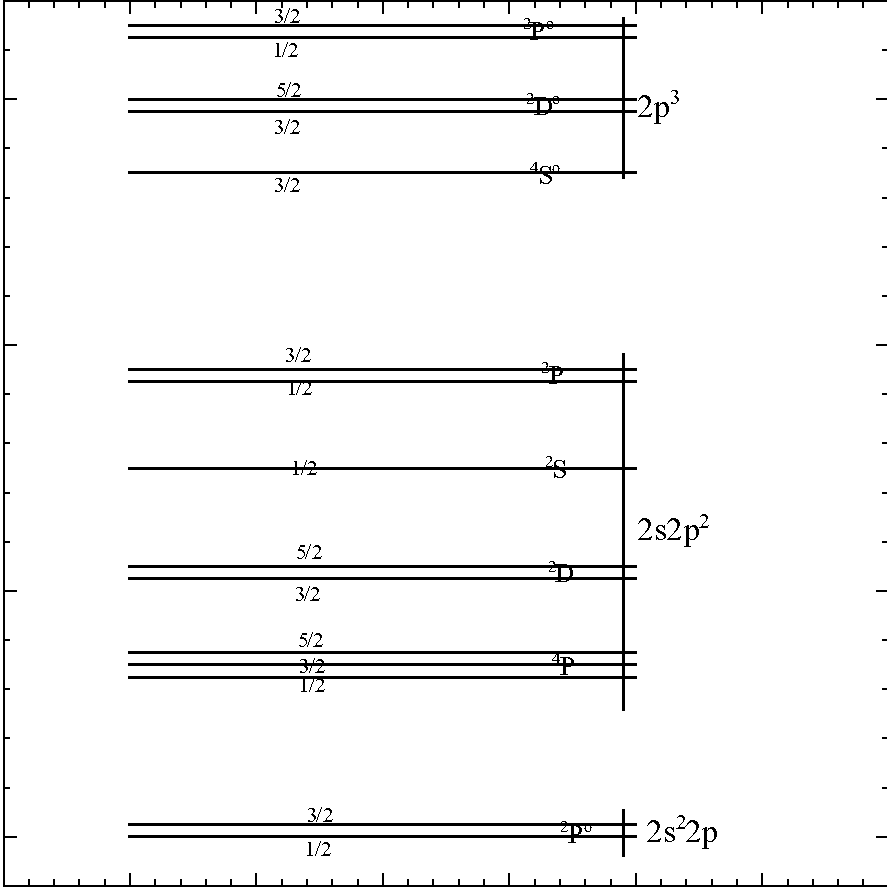
\includegraphics[scale=0.6]{AtomBoronSequence}
\label{fig:AtomBoronSequence}
\caption{Energy Level Diagram for Boron Sequence.}
\end{figure}

\subsection{Beryllium sequence atoms}

Figure \ref{fig:AtomBeSequence} shows the model of the Beryllium sequence.
The level populations, cooling, and line destruction by background opacity
sources are computed for a specialized four level atom in routine
\cdTerm{AtomSeqBeryllium}.

\begin{figure}
\centering
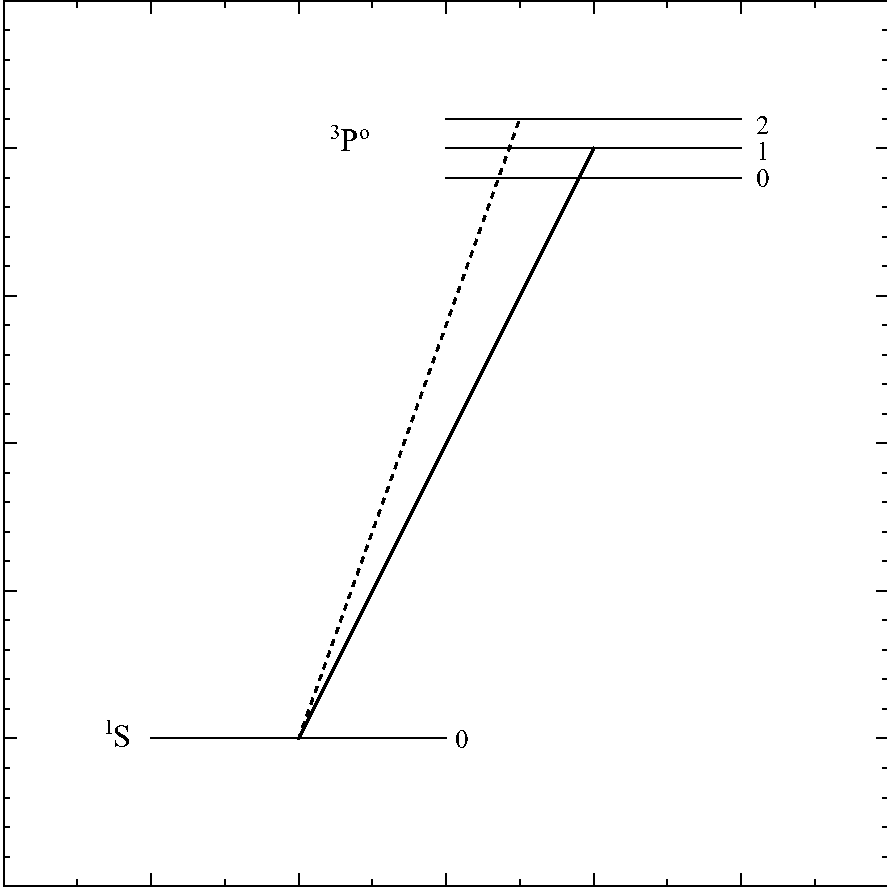
\includegraphics[scale=0.5]{AtomBeSequence}
\label{fig:AtomBeSequence}
\caption{Energy Level Diagram for Beryllium Sequence.}
\end{figure}

Routine \cdTerm{beseq} is called with five arguments, the collision strengths
between the excited triplet levels, the line optical depth array for the
fast $(j=1$ to $j=0)$ transition, and the transition probability for the slow
$(j=2$ to $j=0)$ transition. Induced processes are only included for the fast
transition.   The collision strength stored in the line array is the
collision strength for the entire multiplet.  Rates to levels within the
term are assumed to scale as the ratio of level statistical weight to term
statistical weight.  The level populations for the ground and excited states,
with no correction for stimulated emission, are returned in the array
\cdTerm{PopLevls}, contained in the common block of the same name.

The total rates between any two levels $i\Lambda j$
is indicated by $R_{ij}$.  This
includes collisions, radiative decays (for the fast transition, both photon
escape and destruction by background opacity, and induced transitions).
If the total abundance of the parent ion is $A$, the three balance equations
are
\begin{equation}
{n_0} + {n_1} + {n_2} + {n_3} = A
\end{equation}
\begin{equation}
{n_0}\left( {{R_{01}} + {R_{02}} + {R_{03}}} \right) = {n_1}{R_{10}} +
{n_2}{R_{20}} + {n_3}{R_{30}}
\end{equation}
\begin{equation}
{n_1}\left( {{R_{10}} + {R_{12}} + {R_{13}}} \right) = {n_3}{R_{31}} +
{n_2}{R_{21}} + {n_0}{R_{01}}.
\end{equation}
\begin{equation}
{n_2}\left( {{R_{20}} + {R_{21}} + {R_{23}}} \right) = {n_3}{R_{32}} +
{n_1}{R_{12}} + {n_0}{R_{02}} .
\end{equation}
Collisions are included in all these terms.  $R_{32}$ includes the slow downward
line escape, while $R_{02}$ and $R_{20}$ includes escape, destruction by background
opacity, and fluorescent excitation---deexcitation.  In the code the terms
on the LHS of equations 39, 40, and 38 are called $\alpha$, $\beta$,
and~$\gamma$.

\section{Evaluation of the cooling function}

\subsection{Total cooling}

The cooling function is evaluated in routine \cdTerm{coolr}.  This in turn calls
other routines which compute cooling for individual elements.  Each
individual coolant is entered as a separate quantity in the array
\cdTerm{cooling}.
Under some extreme circumstances agents that are normally coolants can
actually heat the gas.  Negative coolants are stored in a parallel array,
\cdTerm{heatnt}.

The total cooling is the sum of this array, referred to as the variable
\cdTerm{ctot}, and evaluated in routine \cdTerm{SumCool}.

\subsection{The cooling derivative}

As the cooling is evaluated, its approximate temperature derivative is
computed by making analytic expansions of the cooling for individual agents.
For instance, collisionally excited lines of positive ions have collisional
excitation rates that depend on the product
\begin{equation}
{L_{line}} \propto {n_e}{n_{ion}}T_e^{ - 1/2}\exp ( - {T_{exc}}/{T_e})
\end{equation}
where $T_{exc}$ is the excitation temperature of the line.  In this case the
derivative of the cooling function can be expressed as
\begin{equation}
\frac{{d{L_{line}}}}{{dT}} \propto {n_e}{n_{ion}}\frac{d}{{d{T_e}}}T_e^{
- 1/2}\exp ( - {T_{exc}}/{T_e}) = {L_{line}}\left[
{\frac{{{T_{exc}}}}{{T_e^2}} - \frac{1}{{2{T_e}}}} \right]
\end{equation}
This derivative is used by the thermal predictor-corrector routine to make
the initial guess at a new temperature.  This is approximate since both
electron and ionic densities also depend on the temperature.

\section{Evaluation of the heating function}

Various contributions to the heating function are evaluated throughout
the code.  Each heating agent stores its contribution to the total heating
within a cell of the two dimensional array \emph{heating}.   The total heating
is always the sum of the total contents of the \emph{heating} array.

\section{Equilibrium calculations}

This is largely taken after \citet{Ferland1988}.

\subsection{Hydrogen only}

Figure \ref{fig:HydrogenRadiationSTE} shows the results of a series of calculations in which the full
set of statistical and thermal equilibrium equations are solved for thin
cells of pure hydrogen gas with various densities.

\begin{figure}
\centering
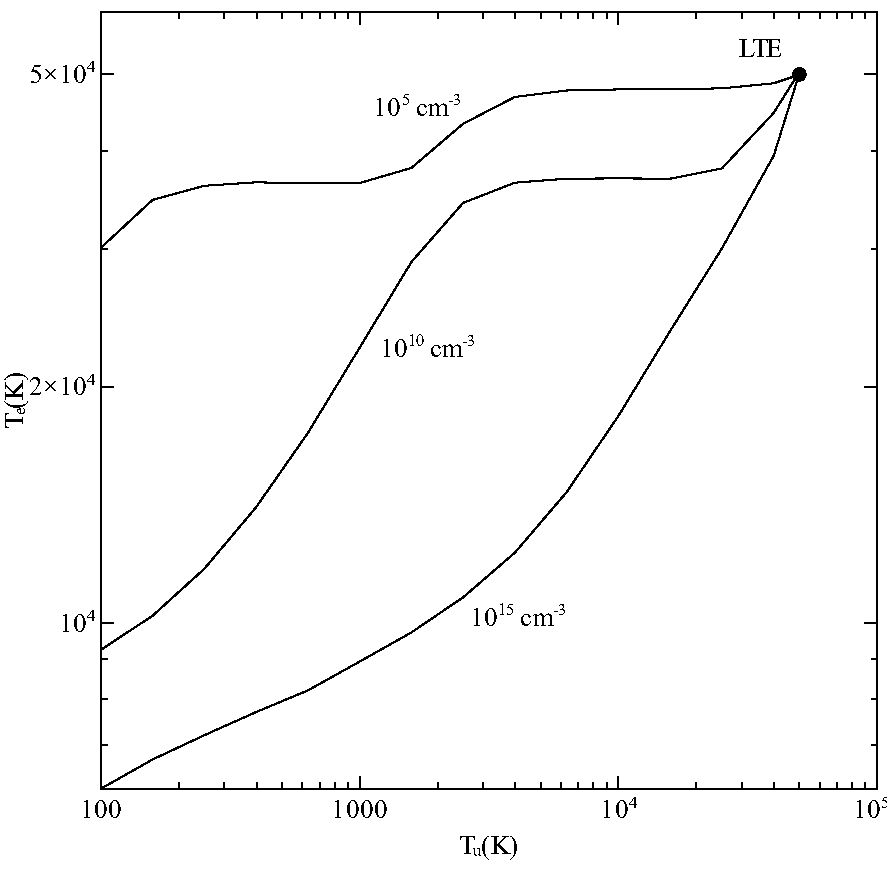
\includegraphics[scale=0.9]{HydrogenRadiationSTE}
\label{fig:HydrogenRadiationSTE}
\caption[Pure hydrogen approach to STE]{Thermal equilibrium calculations for an optically thin gas with
3 hydrogen densities are shown as a function of the radiation field energy
density, parameterized as $T_u$.  Ionization is by a $5 \times 10^4$ K black body.
Various processes drive the gas to thermodynamic equilibrium when $T_u$ reaches
$5\times 10^4$~K.}
\end{figure}

The ionizing continuum is, in all cases,
a black body with $T_{color} = 5\times 10^4 \K$,
and the energy density of the radiation field is varied, up to the
thermodynamic equilibrium limit, $T_u = T_{color}$.

Although the gas temperature in the thermodynamic equilibrium limit does
not depend on the gas density, the physical processes that drive the gas
to this temperature do.  Thermal equilibrium calculations were performed
with three densities chosen to span a fairly wide range.  For low densities
$(n(H) = 10^5$~cm$^{-3}$) the gas remains highly ionized for all values of
$T_u$ shown.
The temperature in thermodynamic equilibrium is set by the balance between
Compton and inverse-Compton scattering.  The intermediate density case $(n(H)
= 10^{10}$ cm$^{-3}$) reaches thermodynamic equilibrium with $\sim$3/4 of the
heating-cooling set by Compton scattering and the remainder due to free-free
and free-bound processes.  The high-density $(n(H) = 10^{15}$ cm$^{-3}$) case reaches
its thermodynamic equilibrium temperature with a balance between free-free
(1/3 of the total) and free-bound (2/3 of the total) processes.  In all
cases the level populations and electron temperature are within $\sim$1\% of their
expected thermodynamic equilibrium values when $T_u = T_{color}$.

\subsection{Helium-only gas}

To do \dots.

\subsection{Metal rich gas}

Simulations of very metal rich gas has been a major emphasis of the code
as described by \citep{Hamann1993} and
\citep{Ferland1996}.  In these cases the thermal
and ionization balance is totally dominated by the heavy elements.

Figure \ref{fig:HighMetalsLTE} shows the results of a series of calculations in which gas with
strongly enhanced abundances of the heavy elements is exposed to a series
of black body radiation fields with different temperatures and energy
densities.   \citep{Ferland1988} and \citep{Ferland1989} gave
analogous calculations for pure hydrogen clouds.  The filled circles
represent the cases where the energy densities of the radiation field are
equal to the color temperature, and strict thermodynamic equilibrium is
expected.  This is indeed the case.  The distribution of ionization for
each color temperature is radically different, but the line interactions
with the radiation field bring the gas to the expected equilibrium
temperature.  This tests both the ionization and thermal balance in this
extreme environment.

\begin{figure}
\centering
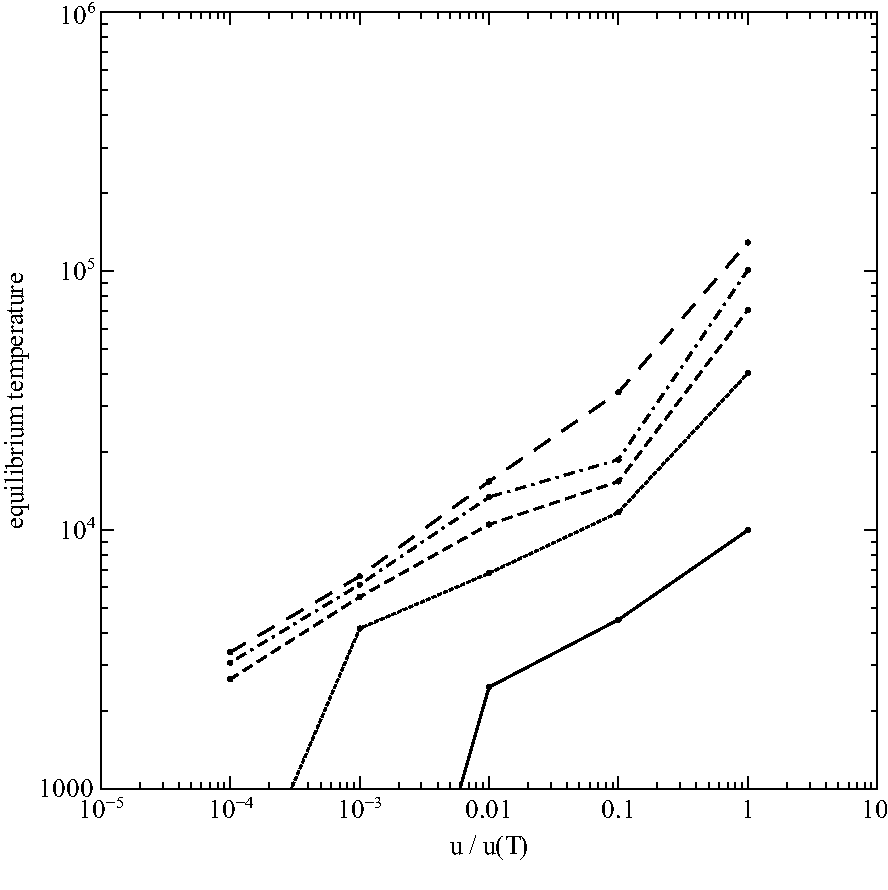
\includegraphics[scale=0.9]{HighMetalsLTE}
\label{fig:HighMetalsLTE}
\caption[High metallicity gas approach to LTE]
{Equilibrium temperature of gas exposed to five black bodies with
various energy density temperatures.  The color temperatures of the
blackbodies are 10000 K, 40000 K, 70000 K, 100000 K and 130000 K.  The
metallicity was 10 times solar (Hamann and Ferland 1993) so that heating
cooling of thousands of heavy element emission lines dominates the thermal
equilibrium.  The simulation is of an optically thin cell of gas with density
$10^{10}$ cm$^{-3}$ (results do not depend on this density).  The x-axis is the local
energy density relative to the energy density in thermodynamic equilibrium
at that temperature.  The gas goes to thermodynamic equilibrium when the
radiation field does (the color and energy density temperatures are equal).}
\end{figure}

